\documentclass[]{report}
\title{API on Rails}
\author{Alexandre Rousseau}

\usepackage{graphicx}
\usepackage{hyperref}
\usepackage[utf8]{inputenc}
\usepackage[french]{babel}
%\usepackage{listings}
\usepackage{appendix}
\usepackage{csquotes}
\usepackage{tcolorbox}
\usepackage{listings}

\showboxdepth=\maxdimen

\pagestyle{headings}

% \hypersetup{
%     colorlinks,
%     citecolor=black,
%     filecolor=black,
%     urlcolor=black
% }

\begin{document}


\maketitle

\newpage

\tableofcontents
\newpage

\pagenumbering{arabic}

\chapter{Droits d'auteur et licence}

  API on rails : Construction d'API REST avec rails. Copyright © 2014 par Abraham Kuri. Tout le code source du tutoriel est disponible conjointement sous la [licence MIT](http://opensource.org/licenses/MIT) et la [licence Beerware](http://people.freebsd.org/~phk/).

  \begin{scriptsize}[breaklines]
  \begin{lstlisting}
  The MIT License

  Copyright (c) 2014 Abraham Kuri

  Permission is hereby granted, free of charge, to any person obtaining a copy
  of this software and associated documentation files (the "Software"), to deal
  in the Software without restriction, including without limitation the rights
  to use, copy, modify, merge, publish, distribute, sublicense, and/or sell
  copies of the Software, and to permit persons to whom the Software is
  furnished to do so, subject to the following conditions:

  The above copyright notice and this permission notice shall be included in
  all copies or substantial portions of the Software.

  THE SOFTWARE IS PROVIDED "AS IS", WITHOUT WARRANTY OF ANY KIND, EXPRESS OR
  IMPLIED, INCLUDING BUT NOT LIMITED TO THE WARRANTIES OF MERCHANTABILITY,
  FITNESS FOR A PARTICULAR PURPOSE AND NONINFRINGEMENT.  IN NO EVENT SHALL THE
  AUTHORS OR COPYRIGHT HOLDERS BE LIABLE FOR ANY CLAIM, DAMAGES OR OTHER
  LIABILITY, WHETHER IN AN ACTION OF CONTRACT, TORT OR OTHERWISE, ARISING FROM,
  OUT OF OR IN CONNECTION WITH THE SOFTWARE OR THE USE OR OTHER DEALINGS IN
  THE SOFTWARE.
  \end{lstlisting}
  \end{scriptsize}

  \begin{scriptsize}
  \begin{lstlisting}
  /*
   * ----------------------------------------------------------------------------
   * "THE BEER-WARE LICENSE" (Revision 42):
   * Abraham Kuri wrote this code. As long as you retain this notice you
   * can do whatever you want with this stuff. If we meet some day, and you think
   * this stuff is worth it, you can buy me a beer in return.
   * ----------------------------------------------------------------------------
   */
 \end{lstlisting}
 \end{scriptsize}

\chapter{Introduction}

  Bienvenue sur APIs on Rails, un tutoriel sous stéroïdes sur la façon de construire votre prochaine API avec Rails. Le but de ce livre est de fournir une réponse sur la façon de développer une API RESTful en suivant les meilleures pratiques existantes. Lorsque vous en aurez fini avec les API Rails, vous devriez être en mesure de créer votre propre API et de l'intégrer à n'importe quel client comme un navigateur Web ou votre une application mobile. Le code généré est construit sur Ruby on Rails 5 qui est la version actuelle, pour plus d'informations à ce sujet, consultez \href{http://rubyonrails.org/}{rubyonrails.org}. La version la plus récente de l'API sur les rails se trouve sur \href{https://apionrails.icalialabs.com}{apionrails.icalialabs.com} ; n'oubliez pas de mettre à jour votre version hors ligne si c'est le cas.

  L'intention de ce livre n'est pas d'enseigner comment construire une API avec Rails, mais plutôt de vous apprendre comment construire une API évolutive et maintenable avec Rails. Ce qui signifie améliorer vos connaissances actuelles Rails  sur cette approche. Dans ce voyage que nous allons faire, vous apprendrez à le faire

  \begin{itemize}
    \item Construire des réponses JSON
    \item Utiliser Git pour le contrôle de version
    \item Test de vos points finaux
    \item Optimiser et mettre en cache l'API
  \end{itemize}

  Je vous recommande fortement d'aller étape par étape sur ce livre. Essayez de ne pas sauter des chapitres car je mentionne des conseils et des faits intéressants pour améliorer vos compétences. Vous pouvez vous considérer comme le personnage principal d'un jeu vidéo et avec chaque chapitre, vous obtiendrez un niveau supérieur.

  Dans ce premier chapitre, je vais vous expliquer comment configurer votre environnement au cas où vous ne l'auriez pas déjà. Nous allons ensuite créer l'application appelée \verb|market_place_api|. Je soulignerai tous mes efforts pour vous enseigner toutes les meilleures pratiques que j'ai apprises au cours des années, ce qui signifie qu'immédiatement après avoir initialisé (Section 1.3) le projet, nous commencerons à le suivre avec Git (Section \ref{setup_git}).

  Dans les prochains chapitres, nous allons construire l'application en suivant un *workflow* simple que j'utilise quotidiennement. Nous développerons toute l'application en utilisant le développement piloté par les tests (TDD), en commençant par expliquer l’intérêt d'utiliser une API pour votre prochain projet et de choisir un format de réponse adapté comme le JSON ou le XML. Du chapitre 3 au chapitre 8, nous mettrons les mains dans le cambouis et nous compléterons les bases de l'application en construisant tous les points finaux nécessaires en sécurisant l'accès à l'API et en gérant l'authentification par échange d'en-têtes. Enfin, dans le dernier chapitre (Chapitre 11), nous ajouterons quelques techniques d'optimisation pour améliorer les réponses du serveur.

  L'application finale grattera la surface pour être une place de marché où les utilisateurs seront en mesure de passer des commandes, télécharger des produits et plus encore. Il existe de nombreuses options pour créer une boutique en ligne comme \href{http://shopify.com/}{Shopify}, \href{http://spreecommerce.com/}{Spree} ou \href{http://magento.com/}{Magento}.

  À la fin ou au cours du processus (cela dépend vraiment de votre expertise), vous allez vous améliorer et être en mesure de mieux comprendre certaines des meilleures ressources Rails. J'ai aussi pris certaines des pratiques que j'ai trouvé et je vous les ai apportées :

  \begin{itemize}
    \item \href{http://railscasts.com/}{Railscasts}
    \item \href{http://codeschool.com/}{CodeSchool}
    \item \href{http://jsonapi.org/format/}{JSON API}
  \end{itemize}

  \section{Conventions sur ce livre}

    Les conventions de ce livre sont basées sur celles du Tutoriel Ruby on Rails. Dans cette section, j'en mentionnerai quelques-unes qui ne sont peut-être pas aussi claires.

    Je vais utiliser de nombreux exemples en utilisant des ligne de commande. Je ne vais pas traiter avec Windows \verb|cmd| (désolé les gars), donc je vais baser tous les exemples en utilisant l'invite de ligne de commande de style Unix, comme suit:

    \begin{scriptsize}
    \begin{lstlisting}[language=bash]
    $ echo "A command-line command"
    A command-line command
    \end{lstlisting}
    \end{scriptsize}

    J'utiliserai quelques lignes directrices relatives au langage Ruby, ce que j'entends par là:

    \begin{itemize}
      \item \textquote{Éviter} signifie que tu n'es pas censé le faire.
      \item \textquote{Préférer} indique que parmi les 2 options, la première est la plus appropriée.
      \item \textquote{Utiliser} signifie que vous êtes en mesure d'utiliser la ressource.
    \end{itemize}

    Si pour une raison quelconque vous rencontrez des erreurs lors de l'exécution d'une commande, plutôt que d'essayer d'expliquer tous les résultats possibles, je vous recommanderai de *"google it"* (ce que je ne considère pas comme une mauvaise pratique). Mais si vous avez envie de prendre une bière ou si vous rencontrez des problèmes avec ce tutoriel, vous pouvez toujours \href{http://twitter.com/kurenn}{me tweeter} ou \href{mailto:kurenn@icalialabs.com}{m'envoyer un email}.

  \section{Pour commencer}

    L'une des parties les plus douloureuses pour presque tous les développeurs est de tout mettre en place, mais tant que vous le faites, les prochaines étapes devraient être un jeu d'enfant et bien récompensé. Afin de vous faciliter la tâche et de vous motiver, nous utiliserons un script bash que je gère, appelé Kaishi, qui inclut tous les outils nécessaires (encadré 1.1) et plus encore pour configurer votre environnement de développement, il ne fonctionne actuellement que pour Mac OS:

    \begin{tcolorbox}{Outils de développement Kaishi}
      \begin{itemize}
        \item \href{https://github.com/robbyrussell/oh-my-zsh}{oh-my-zsh}  en tant que Shell par défault
        \item \href{http://brew.sh/}{Homebrew} pour la gestion des paquets
        \item \href{http://git-scm.com/}{Git} en tant que gestionnaire de base de données
        \item \href{http://www.postgresql.org/}{Postresql} en tant que gestionnaire de base de données
        \item \href{http://www.vim.org/}{Vim} pour l'édition de texte
        \item \href{http://www.imagemagick.org/}{ImageMagick} pour le traitement d'images
        \item \href{https://github.com/sstephenson/rbenv}{Rbenv} pour la gestion de l'environnement rubis
        \item \href{http://bundler.io/}{Bundler}
        \item \href{https://github.com/ddollar/foreman}{Foreman} pour l'exécution d'applications
        \item \href{http://rubyonrails.org/}{Rails} pour la création de n'importe quelle application rails
        \item \href{https://toolbelt.heroku.com/}{Heroku} pour interagir avec l'API Heroku
        \item \href{https://github.com/IcaliaLabs/railsAppCustomGenerator}{RailsAppCustomGenerator} pour initialiser n'importe quelle application Rails avec le modèle d'Icalia
        \item \href{http://pow.cx/}{Pow} pour exécuter des applications locales en local comme un super-héros
      \end{itemize}
    \end{tcolorbox}

  \section{Environnements de développement}

    \subsection{Editeurs de texte et Terminal}

      Il existe de nombreux cas dans lesquels les environnements de développement peuvent différer d'un ordinateur à l'autre. Ce n'est pas le cas avec les éditeurs de texte ou les IDE. Je pense que pour le développement de Rails un IDE est beaucoup trop lourd tandis que d'autres pourraient trouver que c'est la meilleure façon de développer. Si c'est votre cas, je vous recommande d'essayer avec \href{http://www.aptana.com/products/radrails}{RadRails} ou \href{http://www.jetbrains.com/ruby/index.html}{RubyMine}, les deux sont bien soutenus et possèdent de nombreuses intégrations par défault.

      Maintenant pour ceux qui sont plus comme moi, je peux vous dire qu'il y a beaucoup d'options disponibles que vous pouvez personnaliser via des plugins et plus.

      \begin{description}
        \item[Editeur de texte] J'utilise personnellement \href{http://www.vim.org/}{Vim} comme éditeur par défaut avec \href{https://github.com/carlhuda/janus}{Janus} qui ajoute et gère plusieurs des plugins que vous allez probablement utiliser. Au cas où vous n'êtes pas un fan de Vim comme moi, il y a beaucoup d'autres solutions comme \href{http://www.sublimetext.com/}{Sublime Text} qui est une multiplateforme facile à apprendre et à personnaliser (c'est probablement votre meilleure option), il est fortement inspiré par \href{http://macromates.com/}{TextMate} (disponible uniquement pour Mac OS). Une troisième option est d'utiliser un éditeur de texte plus récent des gars de \href{http://gitub.com/}{Github} appelé \href{https://atom.io/}{Atom}, c'est un éditeur de texte prometteur fait en Javascript. Il est facile à personnaliser pour répondre à vos besoins, faites un essai. N'importe lequel des éditeurs que je vous présente fera le travail, donc je vous laisserai décider lequel vous convient.

        \item[Terminal] Si vous avez décidé d'utiliser \href{http://icalialabs.github.io/kaishi/}{kaishi} pour paramétrer l'environnement, vous remarquerez qu'il définit le shell par défaut à \verb|zsh|, ce que je recommande vivement. Pour le terminal, je ne suis pas un fan de l'application Terminal par défault sous Mac OS. Je recommande \href{http://www.iterm2.com/#/section/home}{iTerm2}, qui est un remplacement de terminal pour Mac OS. Si vous êtes sous Linux, vous avez probablement déjà un beau terminal, mais le défaut devrait fonctionner très bien.
      \end{description}

    \subsection{Navigateur web}

      Quand il s'agit de navigateurs, je dirais \href{https://www.google.com/intl/en/chrome/browser/}{Chrome} immédiatement. Mais d'autres développeurs peuvent dire \href{http://www.mozilla.org/en-US/firefox/new/}{Firefox} ou même \href{https://www.apple.com/safari/}{Safari}. N'importe lequel d'entre eux vous aidera à construire l'application que vous voulez. Ils porposent tous un bon inspecteur pour le DOM, un analyseur de réseau et de nombreuses autres fonctionnalités que vous connaissez peut-être déjà.

    \subsection{Note sur les outils}

      Très bien, je comprends que vous ne voudrez peut-être pas inclure tous les paquets qui viennent avec \href{http://icalialabs.github.io/kaishi/}{kaishi}, et c'est juste, ou peut-être que vous avez déjà quelques outils installés, eh bien je vais vous décrire comment installer le bare bones dont vous avez besoin pour commencer:

    \subsection{Note sur les outils}

      Très bien, je comprends que vous ne voudrez peut-être pas inclure tous les paquets qui viennent avec \href{http://icalialabs.github.io/kaishi/}{kaishi}, et c'est normal. Ou peut-être que vous avez déjà quelques outils installés. Je vais vous décrire comment installer seulment ce dont vous avez besoin pour commencer:

    \subsection{Gestionnaire de paquets}

      \begin{description}
        \item[Mac OS] Il existe de nombreuses options pour gérer la façon dont vous installez les paquets sur votre Mac, comme \href{https://www.macports.org/}{Mac Ports} ou \href{http://brew.sh/}{Homebrew}. Les deux sont de bonnes options, mais je choisirais la dernière, j'ai rencontré moins de problèmes lors de l'installation de logiciels et de sa gestion. Pour installer \verb|brew| il suffit d'exécuter la commande ci-dessous:
        \begin{scriptsize}
        \begin{lstlisting}[language=bash]
        $ ruby -e "$(curl -fsSL https://raw.github.com/Homebrew/homebrew/go/install)"
        \end{lstlisting}
        \end{scriptsize}
        \item[Linux] Vous êtes quasiment prêts! Peu importe si vous utilisez \verb|apt|, \verb|pacman|, \verb|yum|, tant que vous vous sentez à l'aise avec lui et que vous savez comment installer des paquets pour pouvoir continuer à avancer.
      \end{description}

    \subsection{Git}
      \label{setup_git}

      Nous utiliserons beaucoup Git, et vous devriez aussi l'utiliser non seulement pour le but de ce tutoriel mais pour chaque projet.

      \begin{description}
        \item[Mac OS]
          \begin{scriptsize}
          \begin{lstlisting}[language=bash]
          $ brew install git
          \end{lstlisting}
          \end{scriptsize}
        \item[Linux]
          \begin{scriptsize}
          \begin{lstlisting}[language=bash]
          $ sudo apt-get install git
          \end{lstlisting}
          \end{scriptsize}
      \end{description}

    \subsection{Ruby}

      Il existe de nombreuseuses façons d'installer et de gérer Ruby, et maintenant vous devriez probablement avoir une version installée (1.8 si vous êtes sous Mac OS). Pour connaître votre version, tapez simplement:

      \begin{scriptsize}
      \begin{lstlisting}[language=bash]
      $ ruby -v
      \end{lstlisting}
      \end{scriptsize}

      Rails 5 nécessite l'installation de la version 2.2.2 ou supérieure. Pour l'installer, je vous recommande de commencer à utiliser \href{http://rvm.io/}{Ruby Version Manager (RVM)} ou \href{http://rbenv.org/}{rbenv}. Ces outils vous permettrons d'installer plusieurs versions de \verb|ruby|. J'ai récemment changé de RVM à rbenv et c'est super, donc n'importe laquelle de ces deux options que vous choisirez est bonne. Dans ce tutoriel, nous allons utiliser rbenv.

      Note pour Mac OS: si vous utilisez Mac, n'oubliez pas que vous devez avoir installé les \href{https://developer.apple.com/downloads/}{outils en ligne de commande pour Xcode}.


      \subsubsection{Mac OS}

        Pour commencer l'installation de ruby, tapez:

        \begin{scriptsize}
        \begin{lstlisting}[language=bash]
        $ rbenv install 2.1.2
        \end{lstlisting}
        \end{scriptsize}

        Ensuite, vous devez configurer la version de ruby qui vient d'être installée comme version par défaut:

        \begin{scriptsize}
        \begin{lstlisting}[language=bash]
        $ rbenv global 2.1.2
        $ rbenv rehash
        \end{lstlisting}
        \end{scriptsize}

        La commande \verb|rehash| est supposée s'exécuter à chaque fois que vous installez une nouvelle version de Ruby ou une Gem. Cela semble beaucoup ? Jetez un coup d'œil à la formule de brasserie \href{https://github.com/sstephenson/rbenv-gem-rehash}{rbenv-gem-rehash-rehash} pour atténuer ce problème.\footnote{Pour plus d'informations sur la personnalisation ou d'autres types d'installation, consultez la \href{https://github.com/sstephenson/rbenv}{documentation du projet}.}.

      \subsubsection{Linux}

        La première étape est de configurer quelques dépendances pour Ruby:

        \begin{scriptsize}
        \begin{lstlisting}[language=bash]
        $ sudo apt-get update
        $ sudo apt-get install git-core curl zlib1g-dev build-essential libssl-dev \
                            libreadline-dev libyaml-dev libsqlite3-dev sqlite3 \
                            libxml2-dev libxslt1-dev libcurl4-openssl-dev zlib1g-dev \
                            python-software-properties
        \end{lstlisting}
        \end{scriptsize}

        Ensuite, vouss pouvez installer la dernière version de Ruby:

        \begin{scriptsize}
        \begin{lstlisting}[language=bash]
        $ cd
        $ git clone git://github.com/sstephenson/rbenv.git .rbenv
        $ echo 'export PATH="$HOME/.rbenv/bin:$PATH"' >> ~/.bash_profile
        $ echo 'eval "$(rbenv init -)"' >> ~/.bash_profile

        $ git clone git://github.com/sstephenson/ruby-build.git ~/.rbenv/plugins/ruby-build
        $ echo 'export PATH="$HOME/.rbenv/plugins/ruby-build/bin:$PATH"' >> ~/.bash_profile
        $ source ~/.bash_profile

        $ rbenv install 2.5.3
        $ rbenv global 2.5.3
        \end{lstlisting}
        \end{scriptsize}

        Si tout s'est bien passé, il est temps d'installer le reste des dépendances que nous allons utiliser.

      \subsubsection{Gems, Rails et bibliothèques manquantes}

        Tout d'abord, nous mettons à jour les Gems sur l'ensemble du système:

        \begin{scriptsize}
        \begin{lstlisting}[language=bash]
        $ gem update --system
        \end{lstlisting}
        \end{scriptsize}

        Dans la plupart des cas, si vous êtes sous Mac OS, vous devriez installer des bibliothèques supplémentaires:

        \begin{scriptsize}
        \begin{lstlisting}[language=bash]
        $ brew install libtool libxslt libksba openssl
        \end{lstlisting}
        \end{scriptsize}

        Nous installons ensuite les gems nécessaires et ignorons la documentation pour chaque gemme :

        \begin{scriptsize}
        \begin{lstlisting}[language=bash]
        $ printf 'gem: --no-document' >> ~/.gemrc
        $ gem install bundler
        $ gem install foreman
        $ gem install rails -v 5.2
        \end{lstlisting}
        \end{scriptsize}

        Vérifiez que tout fonctionne bien:

        \begin{scriptsize}
        \begin{lstlisting}[language=bash]
        $ rails -v 5.2
        5.2.0
        \end{lstlisting}
        \end{scriptsize}

      \subsubsection{Bases de données}

        Je vous recommande fortement d'installer \href{http://www.postgresql.org/}{Postgresql} pour gérer vos bases de données, mais pour plus de simplicité nous allons utiliser \href{http://www.sqlite.org/}{SQlite}. Si vous utilisez Mac OS, vous devriez être prêt à partir, au cas où vous êtes sous Linux, ne vous inquiétez pas, on vous guide:

        \begin{scriptsize}
        \begin{lstlisting}[language=bash]
        $ sudo apt-get install libxslt-dev libxml2-dev libsqlite3-dev
        \end{lstlisting}
        \end{scriptsize}

        ou

        \begin{scriptsize}
        \begin{lstlisting}[language=bash]
        $ sudo yum install libxslt-devel libxml2-devel libsqlite3-devel
        \end{lstlisting}
        \end{scriptsize}

  \section{Initialisation du projet}

    L'initialisation d'une application Rails doit être assez simple pour vous, si ce n'est pas le cas, voici un tutoriel super rapide (Listing \ref{rails_new}).

    Sachez que nous utiliserons \href{http://rspec.info/}{Rspec} comme suite de test, alors assurez-vous d'inclure l'option \verb|-T| lors de la création de l'application rails.

    \begin{scriptsize}
    \begin{lstlisting}[language=bash, caption={Initialisation du projet avec 'rails new'.}, label={rails_new}]
    $ mkdir ~/workspace
    $ cd workspace
    $ rails new market_place_api -T
    \end{lstlisting}
    \end{scriptsize}

    Comme vous pouvez le deviner, les commandes ci-dessus (Listing \ref{rails_new}) génèreront les éléments indispensables de votre application Rails. La prochaine étape est d'ajouter quelques gems que nous utiliserons pour construire l'api.

    \subsection{Installer Pow ou Prax}\label{subsection:install_pow}

      Vous pouvez vous demander, pourquoi diable voudrais-je installer ce type de paquet? La réponse est simple. Nous allons travailler avec des \href{http://en.wikipedia.org/wiki/Subdomain}{sous-domaines}. \href{http://pow.cx/}{Pow} et \href{https://github.com/ysbaddaden/prax.cr}{Prax} vont nous aider a faire cela très facilement.

      \subsubsection{Installer Pow}

        Pow ne fonctionne que sous Mac OS, mais ne vous inquiétez pas, il existe une alternative qui imite les fonctionnalités sous Linux. Pour l'installer, tapez simplement:

        \begin{scriptsize}
        \begin{lstlisting}[language=bash]
        $ curl get.pow.cx | sh
        \end{lstlisting}
        \end{scriptsize}

        Et c'est tout ce que vous avez à faire. Il suffit d'établir un lien symbolique avec l'application pour configurer l'application Rack.

        D'abord vous allez dans le répertoire \verb|~/.pow|:

        \begin{scriptsize}
        \begin{lstlisting}[language=bash]
        $ cd ~/.pow
        \end{lstlisting}
        \end{scriptsize}

        Ensuite, vous pouvez créer le \href{http://en.wikipedia.org/wiki/Symbolic_link}{lien symbolique}

        \begin{scriptsize}
        \begin{lstlisting}[language=bash]
        $ ln -s ~/workspace/market_place_api
        \end{lstlisting}
        \end{scriptsize}

        N'oubliez pas de changer le répertoire utilisateur pour celui qui correspond au votre. Vous pouvez maintenant accéder à l'application via \href{http://market_place_api.dev/}{http://market\_place\_api.dev}. Votre application devrait être en cours d'exécution comme celle illustrée à la Figure \ref{rails_new}.

      \subsubsection{Installer Pax}

        Pour les utilisateurs de Linux uniquement, \href{https://github.com/ysbaddaden/prax.cr}{Prax} distribue des paquet déjà compilé pour les distribution Debian / Ubuntu. Il suffit donc de télécharger le paquet \verb|.deb| et de l'installer avec \verb|dpkg|.

        \begin{scriptsize}
        \begin{lstlisting}[language=bash, breaklines]
        $ cd /tmp
        $ wget https://github.com/ysbaddaden/prax.cr/releases/download/v0.8.0/prax_0.8.0-1_amd64.deb
        $ sudo dpkg -i prax_0.8.0-1_amd64.deb
        \end{lstlisting}
        \end{scriptsize}

        Ensuite, il ne nous reste plus qu'à lier les applications:

        \begin{scriptsize}
        \begin{lstlisting}[language=bash]
        $ cd ~/workspace/market_place_api
        $ prax link
        \end{lstlisting}
        \end{scriptsize}

        Si vous voulez démarrer le prax server automatiquement, ajoutez cette ligne au fichier \verb|.profile|:

        \begin{scriptsize}
        \begin{lstlisting}
        prax start
        \end{lstlisting}
        \end{scriptsize}

        Lors de l'utilisation de \href{https://github.com/ysbaddaden/prax.cr}{Prax}, vous devez spécifier le port de l'URL, dans ce cas-ci: \href{http://market_place_api.dev:3000/}{http://market\_place\_api.dev:3000}:

        Vous devriez voir l'application en marche, voir Figure \ref{fig:pow_running}.

        \begin{figure}
          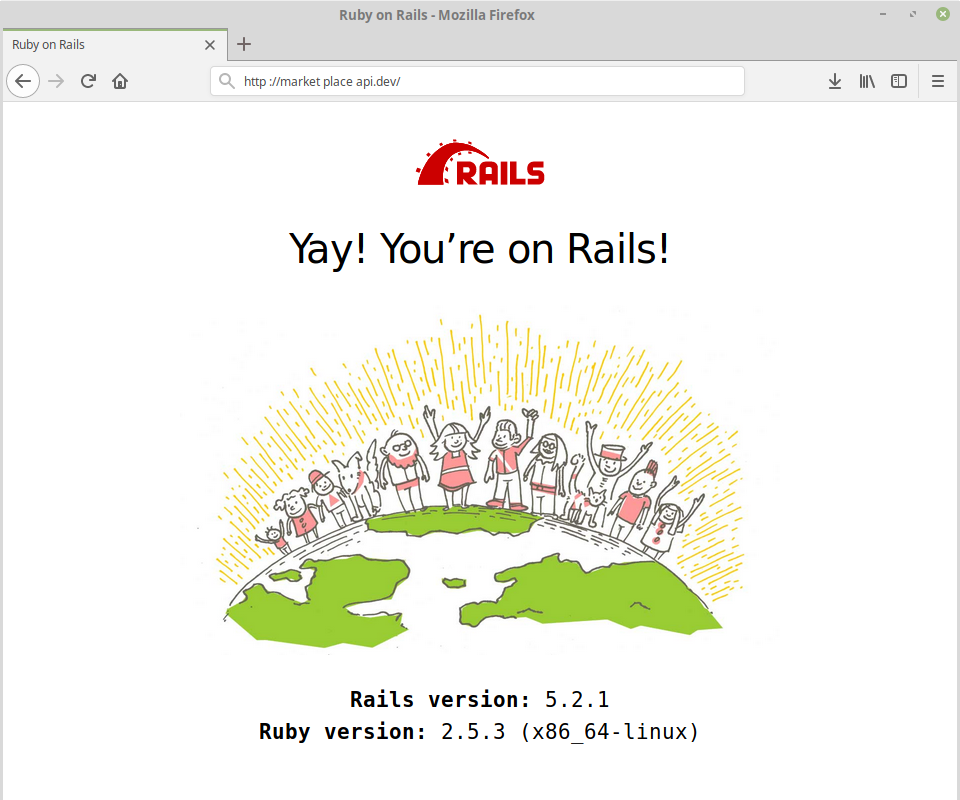
\includegraphics[width=\linewidth]{img/pow_running.png}
          \caption{http://market\_place\_api.dev/}
          \label{fig:pow_running}
        \end{figure}

        Une fois l'application Rails créée, l'étape suivante consiste à ajouter une Gem simple mais très puissante pour sérialiser les ressources que nous allons exposer sur l'API. La Gem s'appelle \verb|active_model_serializers|. C'est un excellent choix pour la construction de ce type d'application car la librairie est bien entretenu et la \href{https://github.com/rails-api/active_model_serializers}{documentation} est incroyable.

        Votre \verb|Gemfile| devrait donc ressembler à ceci (Listing \ref{listing:gemfile_active _model_serializers}) après avoir ajouté la gemme \verb|active _model_serializers|:


        \begin{scriptsize}
        \begin{lstlisting}[language=ruby, caption={Le Gemfile par défaut avec la Gem des sérialiseurs.}, label={listing:gemfile_active _model_serializers}, breaklines]
        source 'https://rubygems.org'
        git_source(:github) { |repo| "https://github.com/#{repo}.git" }

        ruby '2.5.3'

        # Bundle edge Rails instead: gem 'rails', github: 'rails/rails'
        gem 'rails', '~> 5.2.0'
        # Use sqlite3 as the database for Active Record
        gem 'sqlite3'
        # Use Puma as the app server
        gem 'puma', '~> 3.11'
        # Use SCSS for stylesheets
        gem 'sass-rails', '~> 5.0'
        # Use Uglifier as compressor for JavaScript assets
        gem 'uglifier', '>= 1.3.0'

        # Api gems
        gem 'active_model_serializers'

        # ...
        \end{lstlisting}
        \end{scriptsize}

        Notez que j'enlève les gemmes \verb|jbuilder| et \verb|turbolinks| et \verb|coffee-rails|. Nous n'allons pas les utiliser.

        C'est une bonne pratique aussi d'inclure la version ruby utilisée sur l'ensemble du projet, ce qui empêche les dépendances de casser si le code est partagé entre différents développeurs, que ce soit pour un projet privé ou public.

        Il est également important que vous mettiez à jour le Gemfile pour regrouper les différentes gemmes dans l'environnement correct (Listing \ref{listing:gemfile_active _group}) :

        \begin{scriptsize}
        \begin{lstlisting}[language=ruby, caption={Le Gemfile mis à jour pour différents groupes.}, label={listing:gemfile_active _group}, breaklines]
        # ...
        group :development do
          gem 'sqlite3'
        end
        # ...
        \end{lstlisting}
        \end{scriptsize}

        Ceci, comme vous vous en souvenez peut-être, empêchera l'installation ou l'utilisation de sqlite lorsque vous déployez votre application chez un fournisseur de serveurs comme Heroku\footnote{En raison de la structure de l'application, nous n'allons déployer l'application sur aucun serveur, mais nous allons utiliser \href{http://pow.cx/}{Pow} de \href{https://basecamp.com/}{Basecamp}. Si vous utilisez Linux, il existe une solution similaire appelée \href{https://github.com/ysbaddaden/prax.cr}{Prax} par \href{https://github.com/ysbaddaden}{ysbaddaden}. Voir la section \ref{subsection:install_pow}}.

        \begin{displayquote}
          Pow est un serveur Rack zéro-configuration pour Mac OS X. Servez vos applications localement en moins d'une minute. - \href{https://basecamp.com/}{Basecamp}
        \end{displayquote}

        Une fois cette configuration configurée, il est temps d'exécuter la commande d'installation du paquet pour intégrer les dépendances correspondantes:

        \begin{scriptsize}
        \begin{lstlisting}[language=bash, breaklines]
        $ bundle install
        \end{lstlisting}
        \end{scriptsize}

        Une fois que la commande a terminé son exécution, il est temps de commencer à suivre le projet avec git (Section \ref{section:git})

  \section{Contrôle de version}\label{section:git}

    Rappelez-vous que Git vous aide à suivre et à maintenir l'historique de votre code. Gardez à l'esprit que le code source de l'application est publié sur Github. Vous pouvez suivre le référentiel sur \href{https://github.com/madeindjs/market_place_api}{github.com/madeindjs/market\_place\_api}

    À ce stade, je suppose que vous avez déjà configuré git et que vous êtes prêt à l'utiliser pour suivre le projet. Si ce n'est pas votre cas, suivez ces étapes de première installation:

    \begin{scriptsize}
    \begin{lstlisting}[language=bash, breaklines]
    $ git config --global user.name "Type in your name"
    $ git config --global user.email "Type in your email"
    $ git config --global core.editor "vim"
    \end{lstlisting}
    \end{scriptsize}

    Il est donc temps d'initier le projet avec Git. N'oubliez pas de naviguer dans le répertoire racine de l'application \verb|market_place_api|:

    \begin{scriptsize}
    \begin{lstlisting}[language=bash, breaklines]
    $ git init
    Initialized empty Git repository in ~/workspace/market_place_api/.git/
    \end{lstlisting}
    \end{scriptsize}

    L'étape suivante est d'ignorer certains fichiers que nous ne voulons pas suivre. Votre fichier \verb|.gitignore| devrait ressembler à celui montré ci-dessous (Liste ref{lstlisting:gitignore}):

    \begin{scriptsize}
    \begin{lstlisting}[breaklines, caption={La version modifiée du fichier .gitignore}, label={lstlisting:gitignore}]
    # Ignore bundler config.
    /.bundle

    # Ignore the default SQLite database.
    /db/*.sqlite3
    /db/*.sqlite3-journal

    # Ignore all logfiles and tempfiles.
    /log/*
    /tmp/*
    !/log/.keep
    !/tmp/.keep

    # Ignore uploaded files in development
    /storage/*

    /node_modules
    /yarn-error.log

    /public/assets
    .byebug_history

    # Ignore master key for decrypting credentials and more.
    /config/master.key
    \end{lstlisting}
    \end{scriptsize}

    Après avoir modifié le fichier \verb|.gitignore|, il suffit d'ajouter les fichiers et de valider les modifications. Les commandes nécessaires sont indiquées ci-dessous:

    \begin{scriptsize}
    \begin{lstlisting}[language=bash, breaklines]
    $ git add .
    $ git commit -m "Initial commit"
    \end{lstlisting}
    \end{scriptsize}

    Bonne pratique : J'ai appris que commencer un message par un verbe au présent décrit ce que fait le commit et non ce qu'il a fait. De cette façon il est plus facile de lire et de comprendre l'histoirique du projet (ou du moins pour moi). Je vais suivre cette pratique jusqu'à la fin du tutoriel.

    Enfin, comme étape optionnelle, nous installons le projet github (je ne vais pas passer par là) et poussons notre code vers le serveur distant:

    On ajoute d'abord le serveur distant:

    \begin{scriptsize}
    \begin{lstlisting}[language=bash, breaklines]
    $ git remote add origin git@github.com:madeindjs/market_place_api.git
    \end{lstlisting}
    \end{scriptsize}

    ensuite:

    \begin{scriptsize}
    \begin{lstlisting}[language=bash, breaklines]
    $ git push -u origin master
    \end{lstlisting}
    \end{scriptsize}

    Au fur et à mesure que nous avançons dans le tutoriel, j'utiliserai les pratiques que j'utilise quotidiennement. Cela inclut le travail avec les branches, le rebasage, le squash et bien d'autres. Pour l'instant, vous n'avez pas à vous inquiéter si certains des termes ne vous semblent pas familiers, je les expliquerai le temps venu.

  \section{Conclusion}

    Cela a été un long chemin à travers ce chapitre, si vous arrivez ici, permettez-moi de vous féliciter. Soyez sûr que les choses vont s'améliorer à partir de ce point.

    Maintenant, commençons à mettre les mains dans le code!


\end{document}
